\documentclass{report}

\usepackage[utf8]{inputenc}  
\usepackage[T1]{fontenc}    
\usepackage{graphicx}

% Peut etre utile plus tard
% \usepackage[latin1]{inputenc}
% \usepackage[T1]{fontenc}
% \usepackage[francais]{label}

% PAGE DE GARDE
\title{TER - Rendu 1}
\author{Emile Cadorel, Guillaume Gas, Jimmy Furet, Valentin Bouziat}
\date{20 mars 2016}

\begin{document}
\maketitle

\chapter{Introduction}
\section{Présentation de GPGPU}
\cite{ref}
GPGPU (General Purpose on Graphic Processing Units), est un principe informatique visant à utiliser le processeur graphique comme processeur de calcul générique. L’objectif étant de bénéficier de l’architecture massivement parallèle d’un processeur graphique et ainsi résoudre des problèmes pour lesquels nous avons des algorithmes parallèles efficaces.

En effet le processeurs graphique à une capacité de calculs beaucoup plus grande que celle d’un processeur classique. Pour peu qu’il existe un algorithme parallèle pour un problème donné. La programmation GPGPU n’est applicable qu’avec utilisation de drivers et des librairies associées. Ces drivers et librairies généralement proposé par les constructeurs de processeur - Intel, Nvidia, … - permettent la programmation sur la carte pour des informaticiens chevronnés. Il existe deux piliers dans la programmation GPGPU, OpenCL - librairies ouvertes par Kronos Group, et Cuda - développée par Nvidia et nécessitant un GPU Nvidia.

La programmation GPGPU étant d’assez bas-niveaux, il existe des librairies permettant d’abstraire certains principes, comme la gestion mémoire. 

\section{Présentation de SPOC}
SPOC, Stream Processing with OCaml est une bibliothèque qui propose une abstraction pour la programmation GPGPU. Son principal but est de fournir une solution portable, multi-GPGPU, et hétérogène tout en gardant de hautes performances.

Elle permet ainsi l’utilisation des systèmes Cuda/OpenCL avec OCaml, l’unification de ces deux API se faisant via une liaison dynamique, ainsi que d’abstraire également les transferts de données entre le CPU et la carte graphique. 

Enfin, elle permet aussi d’utiliser le typage statique afin de vérifier les noyaux de calcul, écrit en Sarek.

Il existe deux solutions afin d’exprimer les noyaux :
\begin{itemize}

\item Sarek, un langage proche de OCaml : son but étant qu’ils soient simples à exprimer, aient des performances prédictibles, qu’ils soient extensibles, compatibles avec les bibliothèques hautes performances existantes et enfin optimisables.
\item L’interoperabilité avec les noyaux Cuda/OpenCL : permet de réaliser des optimisations supplémentaires, la compatibilité avec les bibliothèques actuelles, mais est moins sûr que Sarek.

\end{itemize}

\section{Présentation des Squelettes de programmation}
Les squelettes de programmation est une forme de programmation avancée permettant de développer des structures dans un code haut-level. Le code écrit s’apparente principalement  à du pseudo-code et permet d’analyser, de compiler ou même de tester du code. Aussi appelé Code Débutant, il permet de simuler des calculs et d’éviter notamment des erreurs de compilations, notamment en permettant à l’utilisateur d’écrire du code en utilisant des structures haut-level tout en évitant certaines limitations imposés par la structure du langage utilisé où tout simplement pour contourner certains problèmes d’ordre algorithmique. De cette façon, il devient plus facile de créer des algorithmes complexes.
Les squelettes de programmation sont notamment très utilisés lors de l’utilisation de design pattern dynamique tel que les templates dans plusieurs langages. Ils sont aussi très utilisés pour permettre de découper le code en structure de données permettant ainsi une lecture plus facile comme avec l’utilisation d'interface, de classe abstraite ou même de méthode virtuelle. Bien d’autres utilisations existes notamment pour faciliter des communications réseaux.

\chapter{Présentation du sujet}

\section{Introduction au domaine}
La programmation GPGPU permet de profiter de l’architecture massivement parallèle du GPU. La GPU possède une architecture SIMD (Single Instruction Multiple Data), proposant de nombreuse unité de calcule. 

Le GPU est decoupé en plusieurs TCP (Texture Processing Cluster), eux-même découper en plusieurs SM. Les SM (Streaming Multi-processor) possèdent une mémoire locale, ils possèdent plusieurs SP (Streaming Processor) permettant des calculs sur nombres flottants, ainsi que des unités SFU (Special Function) Unit permettant le calcul de fonctions spécifiques - cos, sin… . Une mémoire globale est la disposition de chacun des cluster mais est beaucoup plus lentes que la mémoire locale.

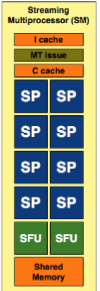
\includegraphics[height=150]{image00.png}
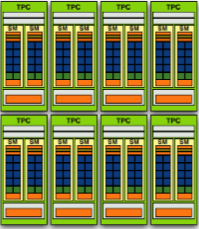
\includegraphics[height=150]{image01.png}


\section{Analyse de l'existant}
Actuellement, la version de SPOC disponible permet déjà d’effectuer des calculs sur la carte graphique, que ce soit en utilisant Cuda ou OpenCL. Elle nous donne également le choix entre l’utilisation de noyaux Sarek ou bien en Cuda/OpenCL. De plus, SPOC met à notre disposition trois bibliothèques, Sarek en faisant partie : 

\begin{itemize}

\item Compose : met à disposition des squelettes (par exemple “map”)
\item Cublas : met à disposition des fonctions de la bibliothèques cuBLAS (Une partie de CUDA Toolkit)
\item Sarek : permet d’exprimer les noyaux

\end{itemize}

\bibliographystyle{plain}
\bibliography{biblio}

\end{document}
